% ****** Start of file apssamp.tex ******
%
%   This file is part of the APS files in the REVTeX 4.1 distribution.
%   Version 4.1r of REVTeX, August 2010
%
%   Copyright (c) 2009, 2010 The American Physical Society.
%
%   See the REVTeX 4 README file for restrictions and more information.
%
% TeX'ing this file requires that you have AMS-LaTeX 2.0 installed
% as well as the rest of the prerequisites for REVTeX 4.1
%
% See the REVTeX 4 README file
% It also requires running BibTeX. The commands are as follows:
%
%  1)  latex apssamp.tex
%  2)  bibtex apssamp
%  3)  latex apssamp.tex
%  4)  latex apssamp.tex
%
\documentclass[%
 reprint,
%superscriptaddress,
%groupedaddress,
%unsortedaddress,
%runinaddress,
%frontmatterverbose, 
%preprint,
%showpacs,preprintnumbers,
%nofootinbib,
%nobibnotes,
%bibnotes,
 amsmath,amssymb,
 aps,
%pra,
%prb,
%rmp,
%prstab,
%prstper,
%floatfix,
spanish]{revtex4-1}

\usepackage{graphicx}% Include figure files
\usepackage{dcolumn}% Align table columns on decimal point
\usepackage{bm}% bold math
\usepackage{subcaption}
\usepackage[utf8]{inputenc}
\usepackage{tabularx}
%\usepackage{hyperref}% add hypertext capabilities
%\usepackage[mathlines]{lineno}% Enable numbering of text and display math
%\linenumbers\relax % Commence numbering lines

%\usepackage[showframe,%Uncomment any one of the following lines to test 
%%scale=0.7, marginratio={1:1, 2:3}, ignoreall,% default settings
%%text={7in,10in},centering,
%%margin=1.5in,
%%total={6.5in,8.75in}, top=1.2in, left=0.9in, includefoot,
%%height=10in,a5paper,hmargin={3cm,0.8in},
%]{geometry}
\graphicspath{ {../} }
\begin{document}

\preprint{APS/123-QED}

\title{Examen computacional sobre Test de Hipótesis\\
  \large Métodos estadísticos en física experimental \\
    No son todos iguales}

\author{A.~Rabinovich (LU:316/08)}
 %\altaffiliation[Also at ]{}%Lines break automatically or can be forced with \\
\affiliation{%
 Departamento de F\'\i sica, Facultad de Ciencias Exactas y Naturales, Universidad de Buenos Aires,\\
 Pabell\'on I, Ciudad Universitaria, 1428 Buenos Aires, Argentina.
}%

%\collaboration{MUSO Collaboration}%\noaffiliation

\date{\today}% It is always \today, today,
             %  but any date may be explicitly specified

\begin{abstract}

\end{abstract}

\maketitle

%\tableofcontents


\section{Introducción}
Sean dos hipótesis especificadas completamente por dos valores distintos de un parámetro $\theta$ en una función de distribución de probabilidad $f(x|\theta)$. 
Para ejemplificar, la hipótesis nula, $H_0$, supone que $\theta = \theta_0$ mientras que la alternativa, $H_1$, asume $\theta = \theta_1$. \\
Suponiendo que la hipótesis nula es cierta, es posible encontrar una región $R$ en el espacio muestral $W$ para la observación $x$ tal que la probabilidad de que $x$ pertenezca a $R$ es igual a algún 
valor numérico asignado previamente. La región R es llamada la región de rechazo o región crítica para $H_0$, mientras que $(W-R)$ es la región de aceptación de $H_0$.\\
Las dos regiones están separadas por un valor $x_c$ y se llama significancia a la probabilidad preasignada de que una observación $x$ pertenezca a $R$. Ésta determina el nivel de significancia 
$100\alpha\%$.\\
\begin{minipage}{0.45\textwidth}									
\centering
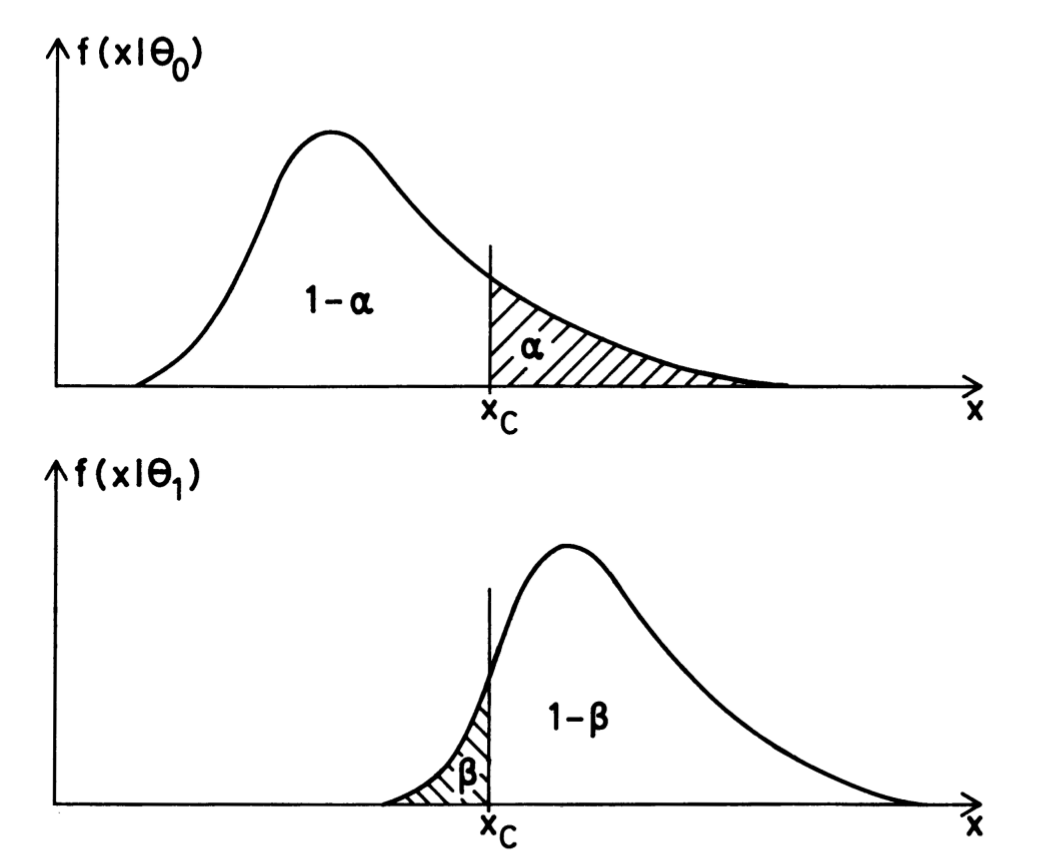
\includegraphics[width=0.9\textwidth]{imagenes/test_de_hipotesis}
\captionof{figure}{Ejemplo de Error de Tipo I, Error de Tipo II y poder de test. Tomado de Frodsen\cite{frodesen}.}
\label{fig:test_de_hipotesis}
\end{minipage}

De ésta definición se desprende que existe una probabilidad $\alpha$ de rechazar $H_0$ cuando era en realidad verdadera, error conocido como Error de Tipo I.\\
Por otro lado, el Error de Tipo II se define como la probabilidad de aceptar $H_0$ cuando era en realidad falsa, y la probabilidad $\beta$ de que ocurra depende de $H_1$\\
Finalmente, el poder de un test se define como la probabilidad $(1-\beta$ de rechazar $H_0$ cuando era realmente falsa. El poder de un test depende de la cantidad de muestras, el nivel de 
significancia y el tamaño del efecto. \\ Todas éstas definiciones se ejemplifican en la figura \ref{fig:test_de_hipotesis}.\cite{frodesen}

\section{El problema}
Sean dos muestras independientes $X_1,...,X_m$ e $Y_1,...,Y_n$ con distribuciones gaussianas $N(\mu_x, \sigma^2)$ y $N(\mu_y, \sigma^2)$ con $\mu_x$, $\mu_y$, $\sigma$ desconocidas.\\
Se quiere estudiar computacionalmente cual de los siguientes test es el de mayor potencia para testear a un nivel de significancia $\alpha$ la hipótesis $H_0$: $\mu_x \leq \mu_x$ contra $H_1$ : 
$\mu_x > \mu_y$.\\
El primero consiste en rechazar $H_0$ cuando $U \geq T_{m+n-2, (1-\alpha)}$, donde:

\begin{equation}
U_1=(\overline{X}-\overline{Y})\sqrt{\frac{m+n-2}{ (\frac{1}{m}+\frac{1}{n})(S_x^2 + S_y^2)  }}
\label{U1}
\end{equation}

con $S_x^2 = \sum_i^m (x_i-\overline{X})^2$ y $S_y^2 = \sum_i^n (y_i-\overline{Y})^2$ y $T_{m+n-2, (1-\alpha)}$ es el cuantil $(1-\alpha)$ de la destribución $T$ con $n+m-2$ grados de libertad.

El segundo consiste en rechazar $H_0$ cuando $U \geq T_{dof, (1-\alpha)}$, donde:

\begin{equation}
U_2=\frac{(\overline{X}-\overline{Y})}{S}
\label{U2}
\end{equation}

con $S^2 = \frac{S_x^2}{m(m-1)} + \frac{S_y^2}{n(n-1)}$ y \\$dof \sim \frac{(\frac{S_x^2}{m(m-1)} + \frac{S_y^2}{n(n-1)})^2}{(\frac{S_x^2}{m(m-1)})^2/(m-1)+(\frac{S_y^2}{n(n-1)})^2/(n-1))}$

\section{Simulaciones}
Se tomaron $m$ muestras para $X \sim N(0.1, 1)$ y $n$ muestras para $Y \sim N(0, 1)$, variando $m$ y $n$ desde 10 hasta 1100 cada una (es decir, en una iteración anidada dentro de la otra) y se 
calcularon los estadísticos $U_1$ y $U_2$. Luego, para cada par $m$ y $n$ se obtuvo el $p-value$ definido como $1-$ la probabilidad acumulada de la $T$ correspondiente hasta $U$. Ésto se repitió 
100 veces y se calculó el promedio del $p-value$ para cada par, como se muestra en la figura \ref{fig:pvalue}.\\
Se observa que los $p-values$ obtenidos con ámbos tests son muy similares, y en ambos casos fue necesario tomar aproximadamente 900 muestras de cada distribución normal para obtener un $p-value < 
0.05$.\\
\begin{figure*}[t]
    \centering
    \begin{subfigure}[t]{0.45\textwidth}
      \centering
      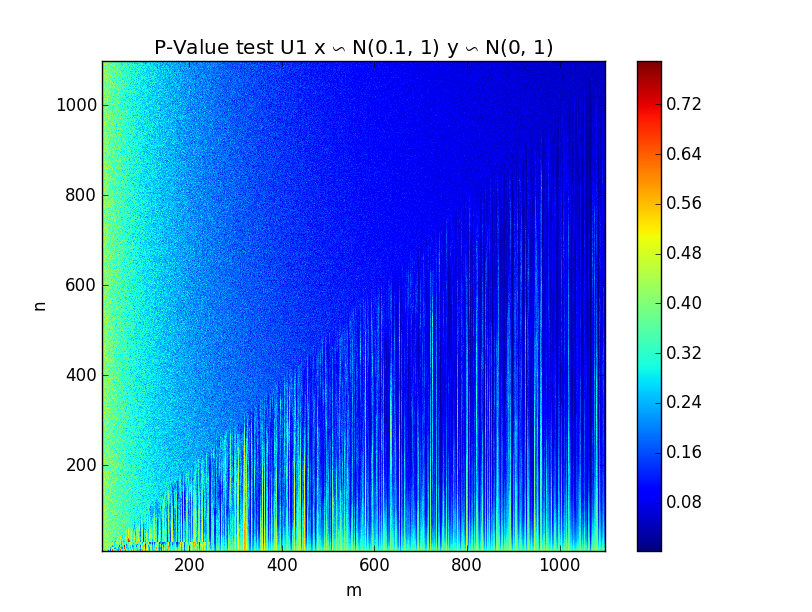
\includegraphics[width=0.9\textwidth]{imagenes/U1_01}
    \end{subfigure}
    \begin{subfigure}[t]{0.45\textwidth}
      \centering
      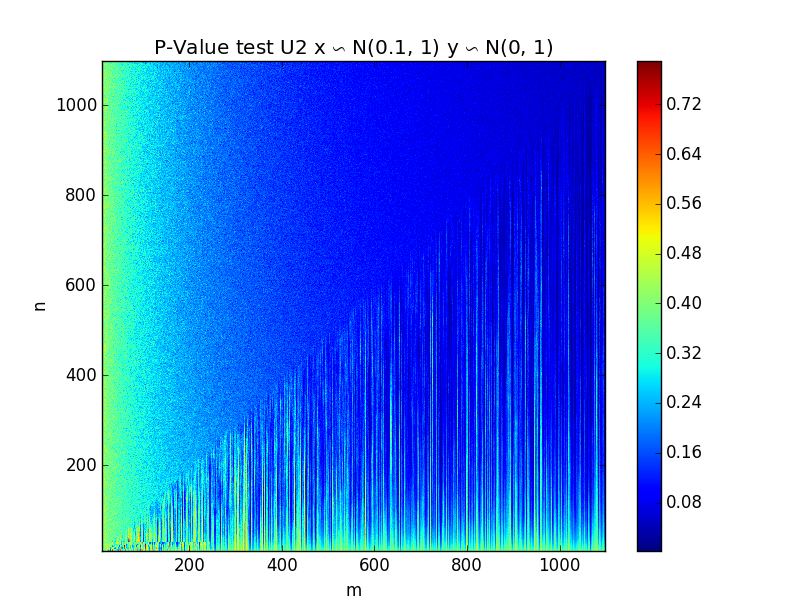
\includegraphics[width=0.9\textwidth]{imagenes/U2_01}
    \end{subfigure}
    \begin{subfigure}[t]{0.45\textwidth}
      \centering
      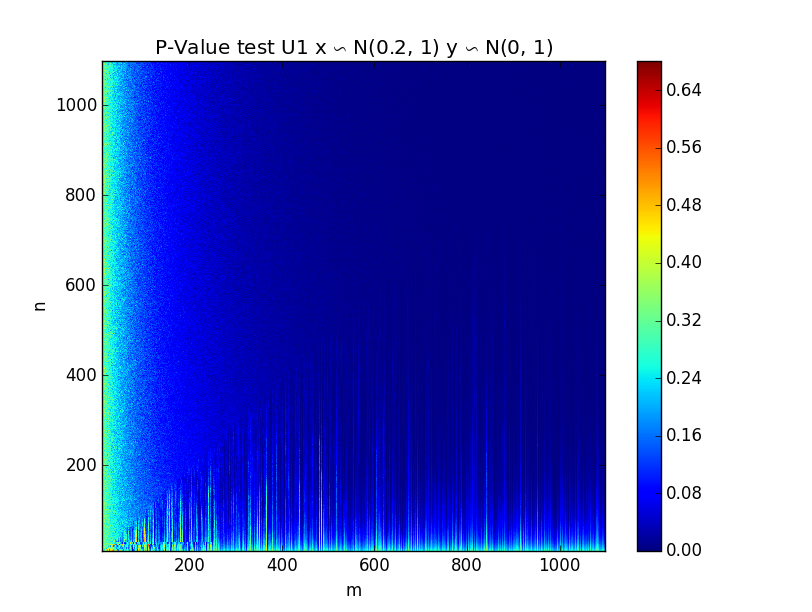
\includegraphics[width=0.9\textwidth]{imagenes/U1_02}
    \end{subfigure}
    \begin{subfigure}[t]{0.45\textwidth}
      \centering
      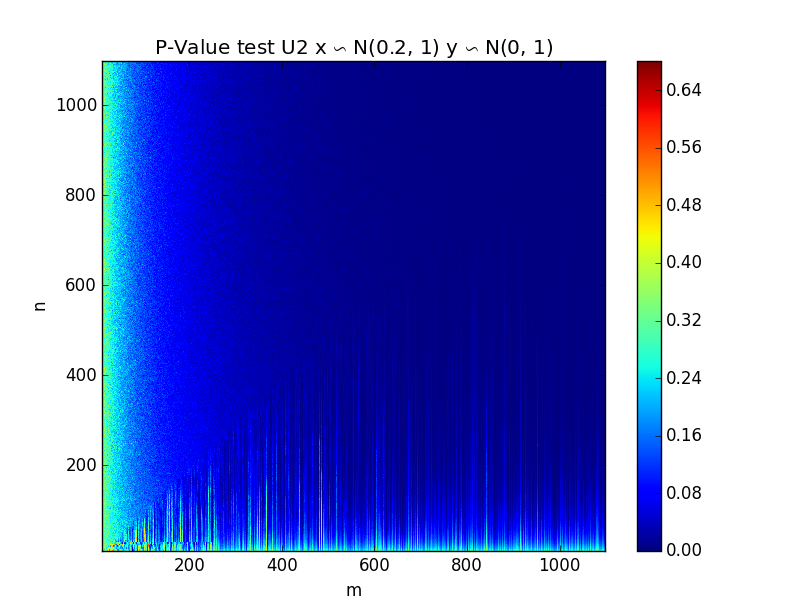
\includegraphics[width=0.9\textwidth]{imagenes/U2_02}
    \end{subfigure} 
    \label{fig:pvalue}
    \caption{P-Value para distintos tests, tamaños de muestra y efectos}
\end{figure*}
Se realizó el mismo proceso tomando muestras de $X \sim N(0.2, 1)$ y graficando el $p-value$, figura \ref{fig:pvalue_02}, y se encontró que con tomar alrededor de 300 muestras de cada distribución 
normal era suficiente. Ésto concuerda con la dependencia del test con el tamaño del efecto. A un efecto mayor (mayor diferencia entre las medias), se requiere una menor cantidad de muestras para 
obtener la significancia necesaria.\\
Por otro lado, se midió el poder de cada test tomando 2000 muestras de $U1$ y $U2$ para cada $n$ y $m$, con $\mu_x > \mu_y$ y con $\mu_x < \mu_y$. En las figuras \ref{fig:histogramas_poder_01} y  
\ref{fig:histogramas_poder_02} se observan histogramas para $n=m=100$, $n=m=500$ y $n=m=900$ para diferencia de medias de 0.1 y $n=m=10$, $n=m=100$ y $n=m=300$ para diferencia de medias de 0.2 
respectivamente. En rojo, $x_c$.

\begin{figure*}[t]
    \centering
    \begin{subfigure}[t]{0.3\textwidth}
      \centering
      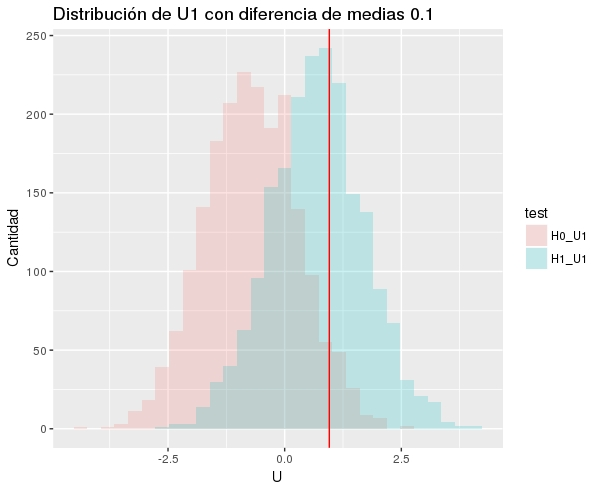
\includegraphics[width=0.9\textwidth]{imagenes/histograma_U1_01_100}
    \end{subfigure}
    \begin{subfigure}[t]{0.3\textwidth}
      \centering
      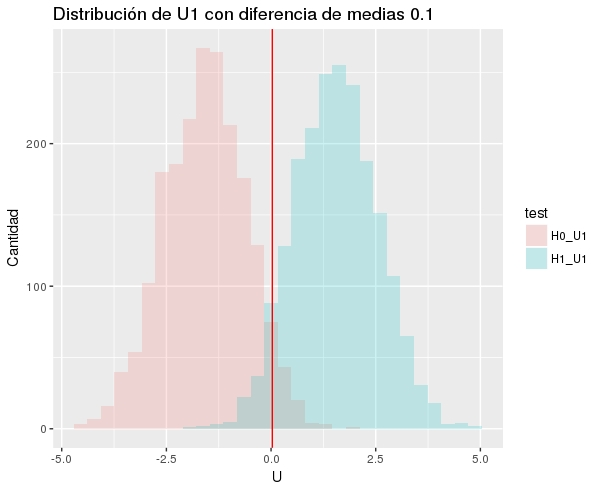
\includegraphics[width=0.9\textwidth]{imagenes/histograma_U1_01_500}
    \end{subfigure}
    \begin{subfigure}[t]{0.3\textwidth}
      \centering
      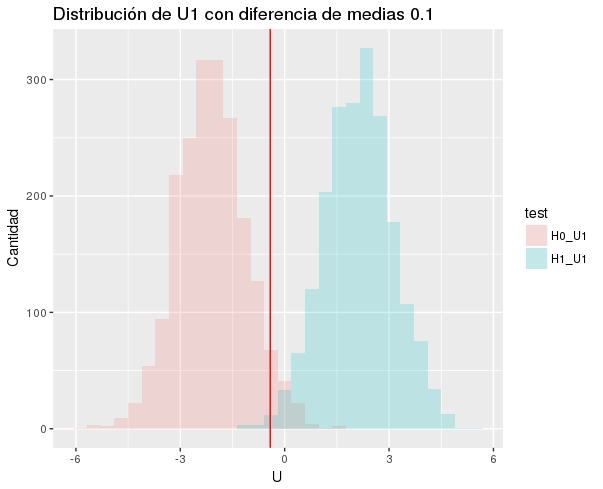
\includegraphics[width=0.9\textwidth]{imagenes/histograma_U1_01_900}
    \end{subfigure}
    \label{fig:histogramas_poder_01}
    \caption{Histogramas de $H_0$ y $H_1$ para test U1 con diferencia de media de 0.1 para n=m con n=100, 500 y 900 respectivamente. Se observa que las distribuciones se separan a medida que aumenta 
el tamaño de la muestra.}
\end{figure*}

\begin{figure*}[t]
    \centering
    \begin{subfigure}[t]{0.3\textwidth}
      \centering
      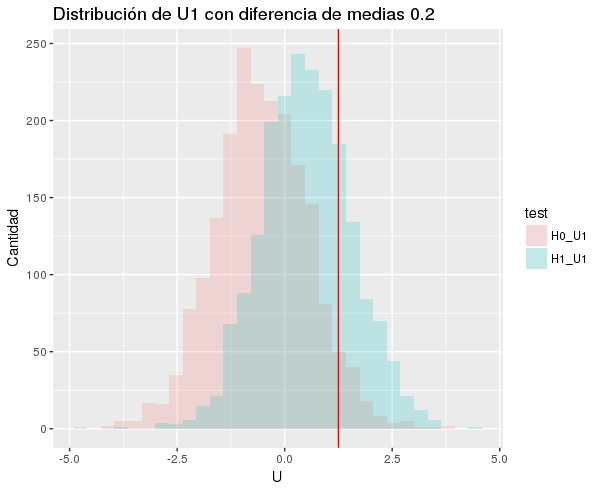
\includegraphics[width=0.9\textwidth]{imagenes/histograma_U1_02_10}
    \end{subfigure}
    \begin{subfigure}[t]{0.3\textwidth}
      \centering
      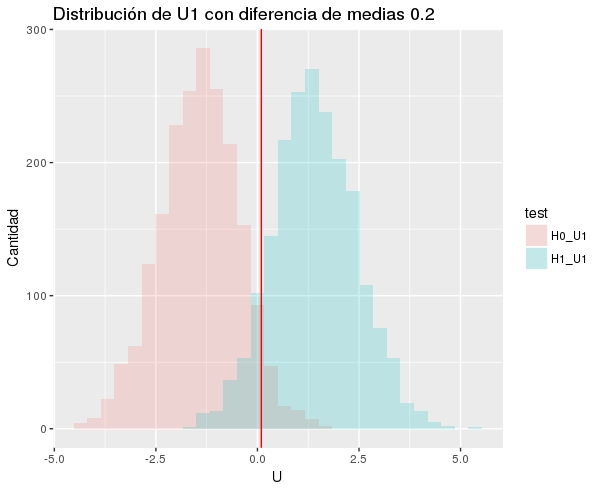
\includegraphics[width=0.9\textwidth]{imagenes/histograma_U1_02_100}
    \end{subfigure}
    \begin{subfigure}[t]{0.3\textwidth}
      \centering
      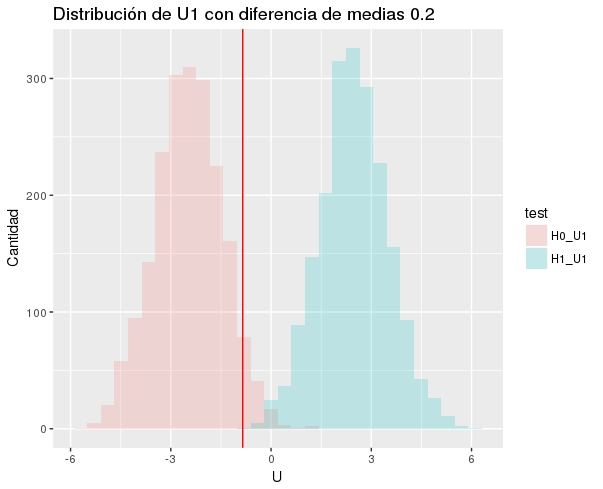
\includegraphics[width=0.9\textwidth]{imagenes/histograma_U1_02_300}
    \end{subfigure}
    \label{fig:histogramas_poder_02}
    \caption{Histogramas de $H_0$ y $H_1$ para test U1 con diferencia de media de 0.2 para n=m con n=10, 100 y 300 respectivamente. Se observa que las distribuciones se separan a medida que aumenta 
el tamaño de la muestra.}
\end{figure*}

Se verifica que a medida que aumenta el tamaño de las muestras, ambas distribuciones se separan. También se observa que a mayor efecto, menor cantidad de muestras alcanza para separar las 
distribuciones. La figura \ref{fig:poder} muestra el poder de cada test y su dependencia con el tamaño de la muestra. Nuevamente, se observa que para tamaños de efecto mayores se requiere de una menor 
cantidad de muestras para conseguir aumentar el poder del test.

\begin{figure*}[t]
    \centering
    \begin{subfigure}[t]{0.45\textwidth}
      \centering
      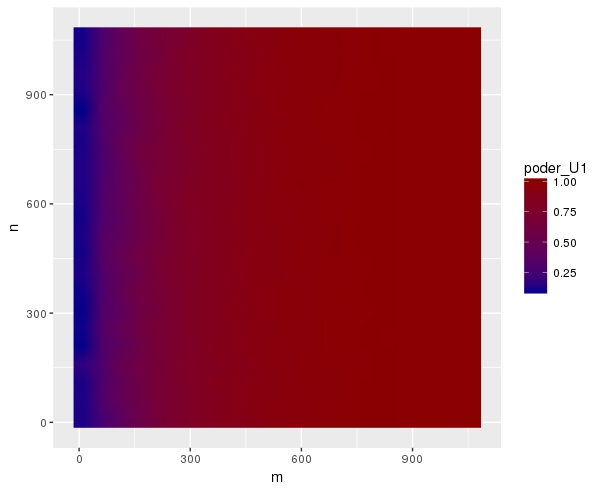
\includegraphics[width=0.9\textwidth]{imagenes/poder_U1_01}
    \end{subfigure}
    \begin{subfigure}[t]{0.45\textwidth}
      \centering
      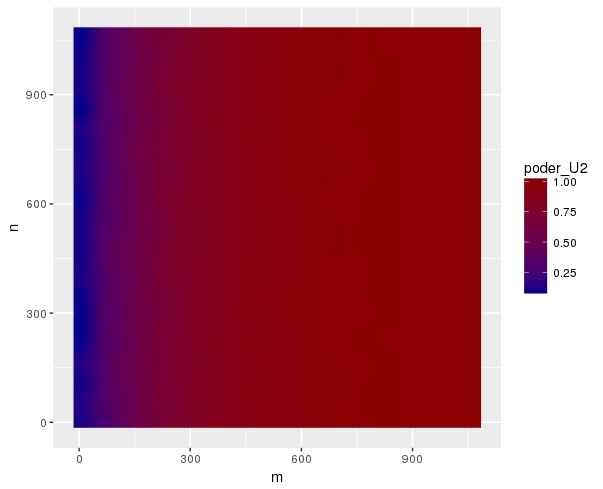
\includegraphics[width=0.9\textwidth]{imagenes/poder_U2_01}
    \end{subfigure}
    \begin{subfigure}[t]{0.45\textwidth}
      \centering
      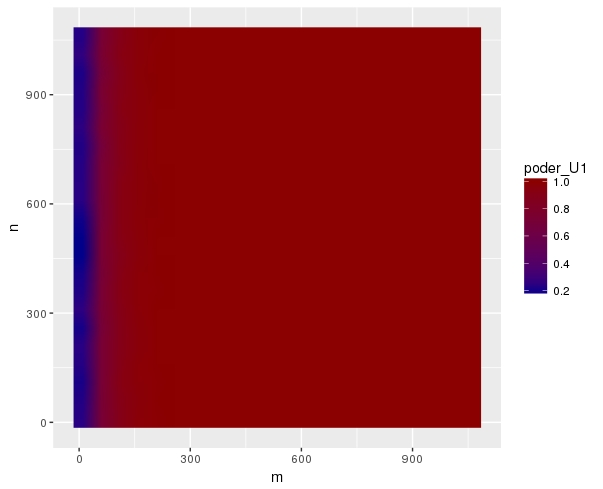
\includegraphics[width=0.9\textwidth]{imagenes/poder_U1_02}
    \end{subfigure}
    \begin{subfigure}[t]{0.45\textwidth}
      \centering
      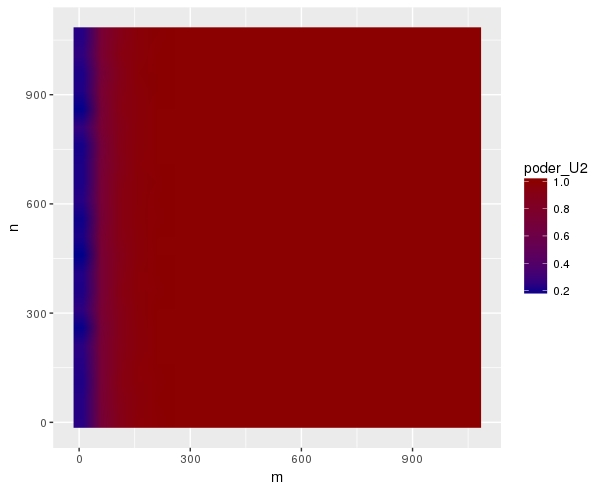
\includegraphics[width=0.9\textwidth]{imagenes/poder_U2_02}
    \end{subfigure} 
    \label{fig:pvalue}
    \caption{Poder para distintos tests, tamaños de muestra y efectos}
\end{figure*}

Se observa además que basta con aumentar el tamaño de las muestras de $x$ para lograr aumentar la potencia del test.

\section{Conclusiones}


\begin{acknowledgments}
A. Rabinovich es becario doctoral del CONICET. 
\end{acknowledgments}

\appendix
\bibliography{examen}% Produces the bibliography via BibTeX.

\end{document}


